\documentclass{article}
\usepackage[utf8]{inputenc}

%Para ver de forma linda el código de C
\usepackage{listings}
\usepackage{color}
\usepackage{amsmath}
\usepackage{graphicx}
%Para ubicar las imagenes entre texto
\usepackage{float}
%Para usar \caption*{} (descripcion sin numerar)
\usepackage{caption}
%Para usar nota al pie dentro de una tabla
\usepackage{footnote}
%Para incluir PDFs
\usepackage[final]{pdfpages}
\usepackage{float}

%Para ver de forma linda el código de C
\usepackage{listings}
\usepackage{color}
\definecolor{listinggray}{gray}{0.9}
\definecolor{lbcolor}{rgb}{0.9,0.9,0.9}

\begin{document}
\begin{titlepage}
\newcommand{\HRule}{\rule{\linewidth}{0.5mm}} % Defines a new command for the horizontal lines, change thickness here

\center % Center everything on the page
 
%----------------------------------------------------------------------------------------
%	HEADING SECTIONS
%----------------------------------------------------------------------------------------

\textsc{\LARGE U.B.A.    FACULTAD DE INGENIER\'IA}\\[1cm] % Name of your university/college
\textsc{\Large Departamento de Electr\'onica \\ Organizaci\'on de Computadoras 66-20\\
Ing. Inform\'atica} \\%[0.5cm] % Major heading such as course name
\textsc{\large }\\%[0.5cm] % Minor heading such as course title

%----------------------------------------------------------------------------------------
%	TITLE SECTION
%----------------------------------------------------------------------------------------

\HRule \\[0.4cm]
{ \huge \bfseries Trabajo pr\'actico Nº01\\ Assembly Mips}\\[0.4cm] % Title of your document
\HRule \\[1.5cm]
 
%----------------------------------------------------------------------------------------
%	AUTHOR SECTION
%----------------------------------------------------------------------------------------
\begin{minipage}{0.4\textwidth}
\begin{flushleft} \large
\emph{Apellido y Nombre:}\\
Cabrera, Jorge\\
Capolupo, Mauro\\
\end{flushleft}
\end{minipage}
~
\begin{minipage}{0.4\textwidth}
\begin{flushright} \large
\emph{Padrón:} \\
93310\\
90283\\
\end{flushright}
\end{minipage}\\[2cm]

\begin{flushleft} \large
{ Fecha de Entrega : 20/09/2016 \\
  Fecha de Reentrega :
  Fecha de Aprobaci\'on :\\
  Calificaci\'on :\\
  Firma de Aprobaci\'on :
}
\end{flushleft}

\vfill % Fill the rest of the page with whitespace

\end{titlepage}

\section{Diseño e implementaci\'on del programa}
\indent El programa implementa un algoritmo sencillo que permite dibujar el conjunto de Julia y sus vecindades, seg\'un un determinadi conjunto de par\'ametros que ser\'an ingresados por l\'inea de comando. 

\subsection{Par\'ametros}
\begin{itemize}
    \item -r: setea la resoluci\'on de la im\'agen generada
    \item -c: especifica el centro de la im\'agen
    \item -C: MAURO NO SE QUE MIERDA HACE ESTA CTE ACLARALO
    \item -w: ancho del ract\'angulo de la regi\'on del plano complejo a dibujar
    \item -H: alto del ract\'angulo de la regi\'on del plano complejo a dibujar
    \item -o: permite colocar la imagen de salida en el archivo pasado como par\'{a}metro o stdout en caso de que el argumento sea '-'
\end{itemize}
 
\section{Comando(s) para compilar el programa en NetBSD}
    gcc -Wall -g -o orga2016TP0 orga2016TP0.c    
\section{Comando(s) para ejecutar el programa en NetBSD}
    ./orga2016TP0 -o Julia.pgm
    
\section{Pruebas}
\subsection{Prueba 1}
Generamos el conjunto Julia con par\'ametros v\'alidos
\begin{center}
    ./orga2016TP0 -r 640x480 -c 1-1i -w 4 -H 2 -o Julia.pgm
\end{center}
\begin{figure}[H]
  \begin{center}
  	\includegraphics[width=100mm]{Julia_test1}
  \end{center}
  \caption{Prueba 1}
\end{figure}

\raggedright
\subsection{Prueba 2}
Generamos el conjunto Julia con par\'ametros v\'alidos
\begin{center}
    ./orga2016TP0 -r 640x480 -c -1-1i -w 4 -H 2 -o Julia.pgm
\end{center}
\begin{figure}[H]
  \begin{center}
  	\includegraphics[width=100mm]{Julia_test2}
  \end{center}
  \caption{Prueba 2}
\end{figure}

\raggedright
\subsection{Prueba 3}
Generamos el conjunto Julia con par\'ametros v\'alidos
\begin{center}
    ./orga2016TP0 -r 480x240 -c -0.1+0.1i -w 4 -H 2 -o Julia.pgm
\end{center}
\begin{figure}[H]
  \begin{center}
  	\includegraphics[width=100mm]{Julia_test3}
  \end{center}
  \caption{Prueba 3}
\end{figure}

\section{Pruebas casos de errores}
\raggedright
\subsection{Prueba 1}
Par\'ametro r inv\'alido
\begin{center}
    ./orga2016TP0 -r 640-480 -c 1-1i -w 4 -H 2 -o Julia.pgm\\
\end{center}
Se esperaba que el caracter delimitador sea 'x'. El mensaje que veremos por pantalla ser\'a:\\
\center
Fatal: invalid r specification.

\raggedright
\subsection{Prueba 2}
Par\'ametro w inv\'alido
\begin{center}
    ./orga2016TP0 -r 640x480 -c 1-1i -w A -H 2 -o Julia.pgm\\
\end{center}
Los valores tanto de 'w' como de 'H' deben ser valores enteros.
\center
Fatal: invalid w specification.

\raggedright
\subsection{Prueba 3}
Par\'ametro c inv\'alido
\begin{center}
    ./orga2016TP0 -r 640x480 -c a-bi -w 2 -H 2 -o Julia.pgm\\
\end{center}
Los valores correspondientes a la parte real e imaginaria del par\'ametro complejo c deben ser reales.
\center
Fatal: invalid c specification.

\newpage
\raggedright
\section{Codigo}
\begin{lstlisting}
\end{lstlisting}

\raggedright
\section{Conclusiones}
\indent Se implement\'o un algoritmo para dibujar el conjunto Julia y sus vecindades, variando los par\'ametros de entrada. Nos familiarizamos con MIPS y las distintas herramientas necesarias para el desarrollo de los siguientes trabajos.

\section{Enunciado}
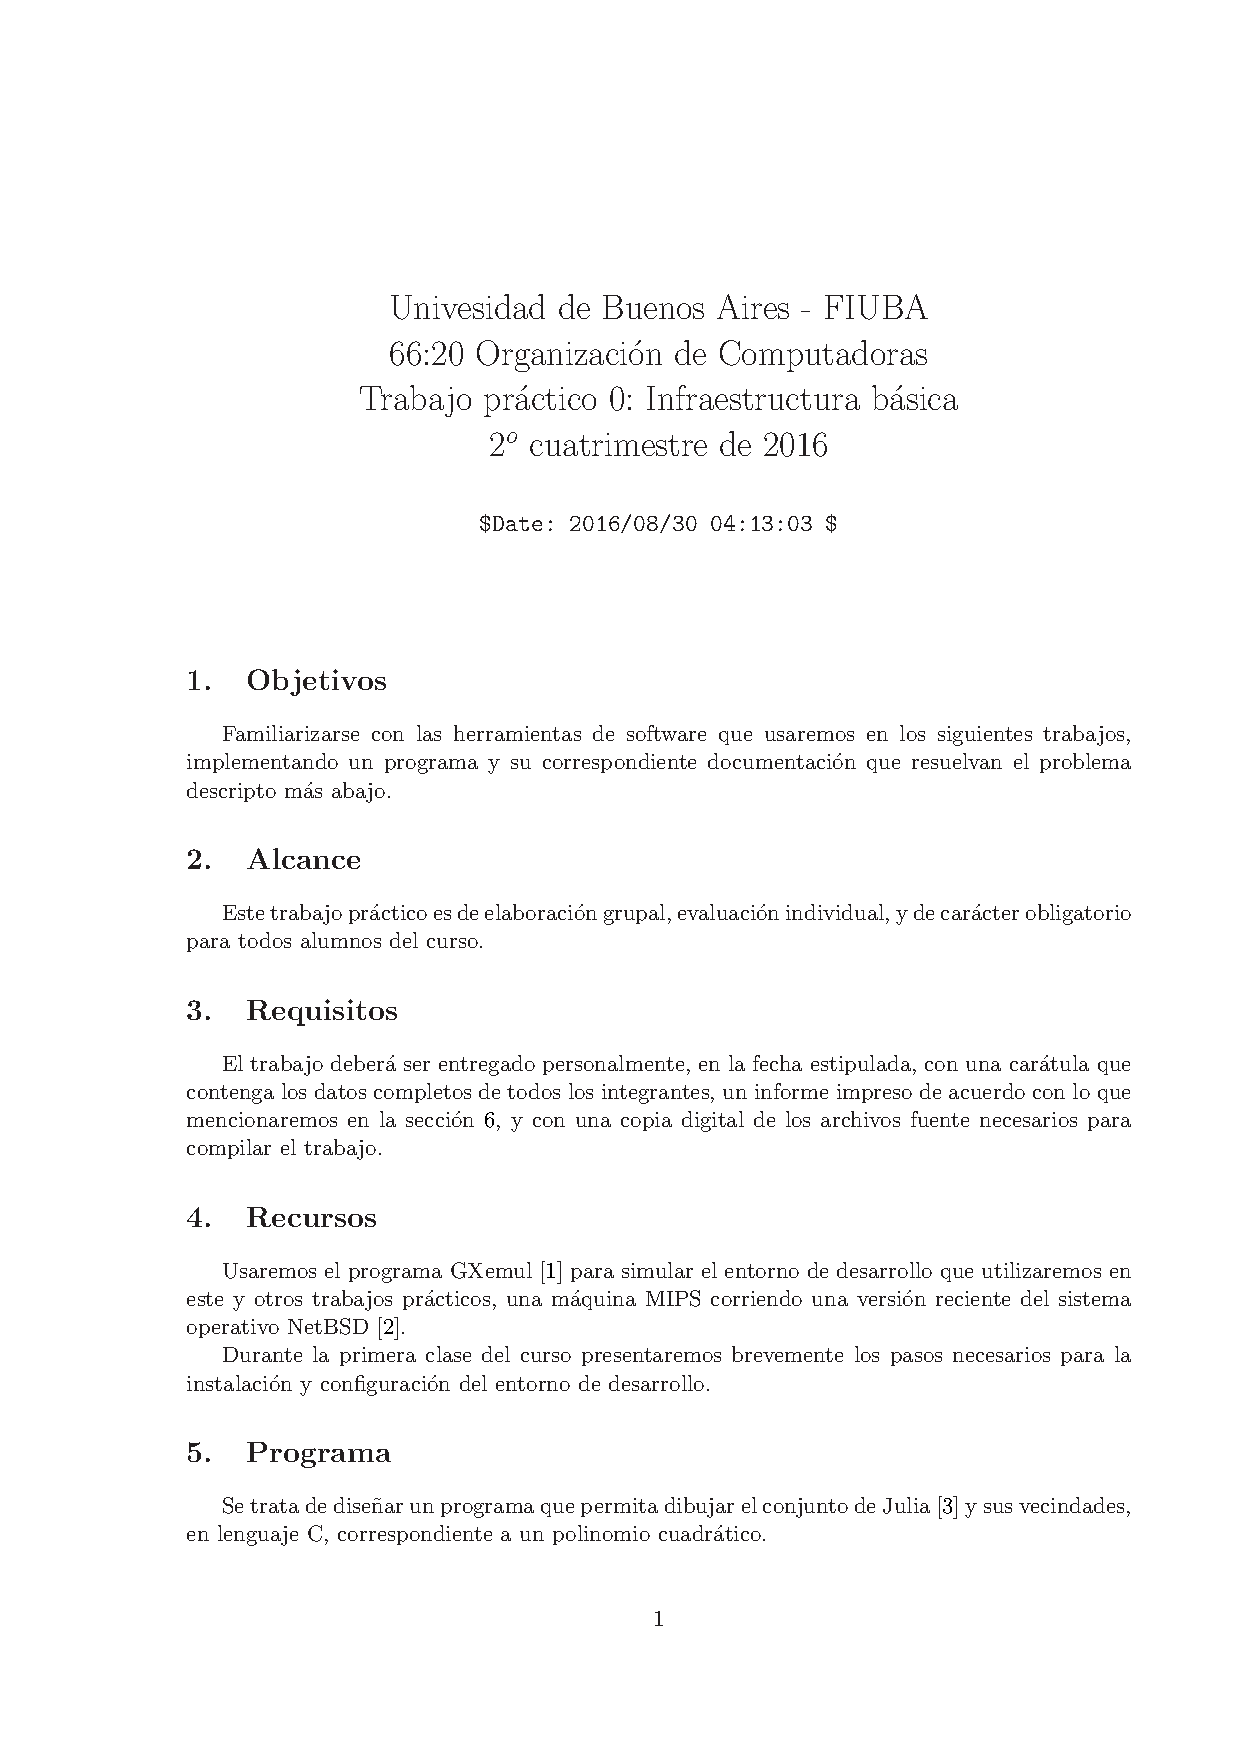
\includepdf[pages=-]{tp0-2016-2q.pdf}

\end{document}